\section{Platine A als Single-Tone Sender}
Für den ersten Teil des Versuchs werden zwei identische Tranceiver Platinen verwendet, die bereits im Verlauf dieses Praktikums genauer betrachtet wurden.
Die beiden Platinen haben folgende Spezifikationen (\textcolor{red}{X} steht hierbei dafür das der Jumper enfernt ist, 
\textcolor{green}{\checkmark} das der Jumper gesetzt ist):\\ 

\begin{table}[h!]
    \centering
    \begin{tabular}{|c|c|c|c|}
        \hline
         & J1 & J2 & Funktion \\
        \hline
        Platine A & \textcolor{red}{X} & \textcolor{green}{\checkmark} & Sender \\
        Platine B &\textcolor{red}{X} & \textcolor{red}{\textbf{X}} & Empfänger \\
        \hline
    \end{tabular}
    \caption{Spezifikationen der beiden Platinen}
    \end{table}
Die folgenden Abbildungen 4.1 und 4.2 zeigen auf der linken Seite die Platine B als Empfänger und auf der rechten Seite
die Platine A als Sender. Die (äußeren Lampen an USB Port) beiden Lampen XX leuchten sobald eine Versorgungsspannung
anliegt. Sind Sender und Empfänger innerhalb der Funkreichweite, so leuchtet weder die Lampe TX (eng. transmitting: senden), noch die Lampe RX (eng. receiving: empfangen) am Sender und Empfänger.
Ist die Funkreichweite überschritten, so leuchtet die Lampe RX am Sender, die Lampe TX leuchtet nicht. Die Lampen
TX und RX am Empfänger leuchten weiterhin nicht. Der Versuch bestätigt hiermit unser Grundlegendes Verständnis 
der Schaltung.

\begin{figure}[H]
    \centering
    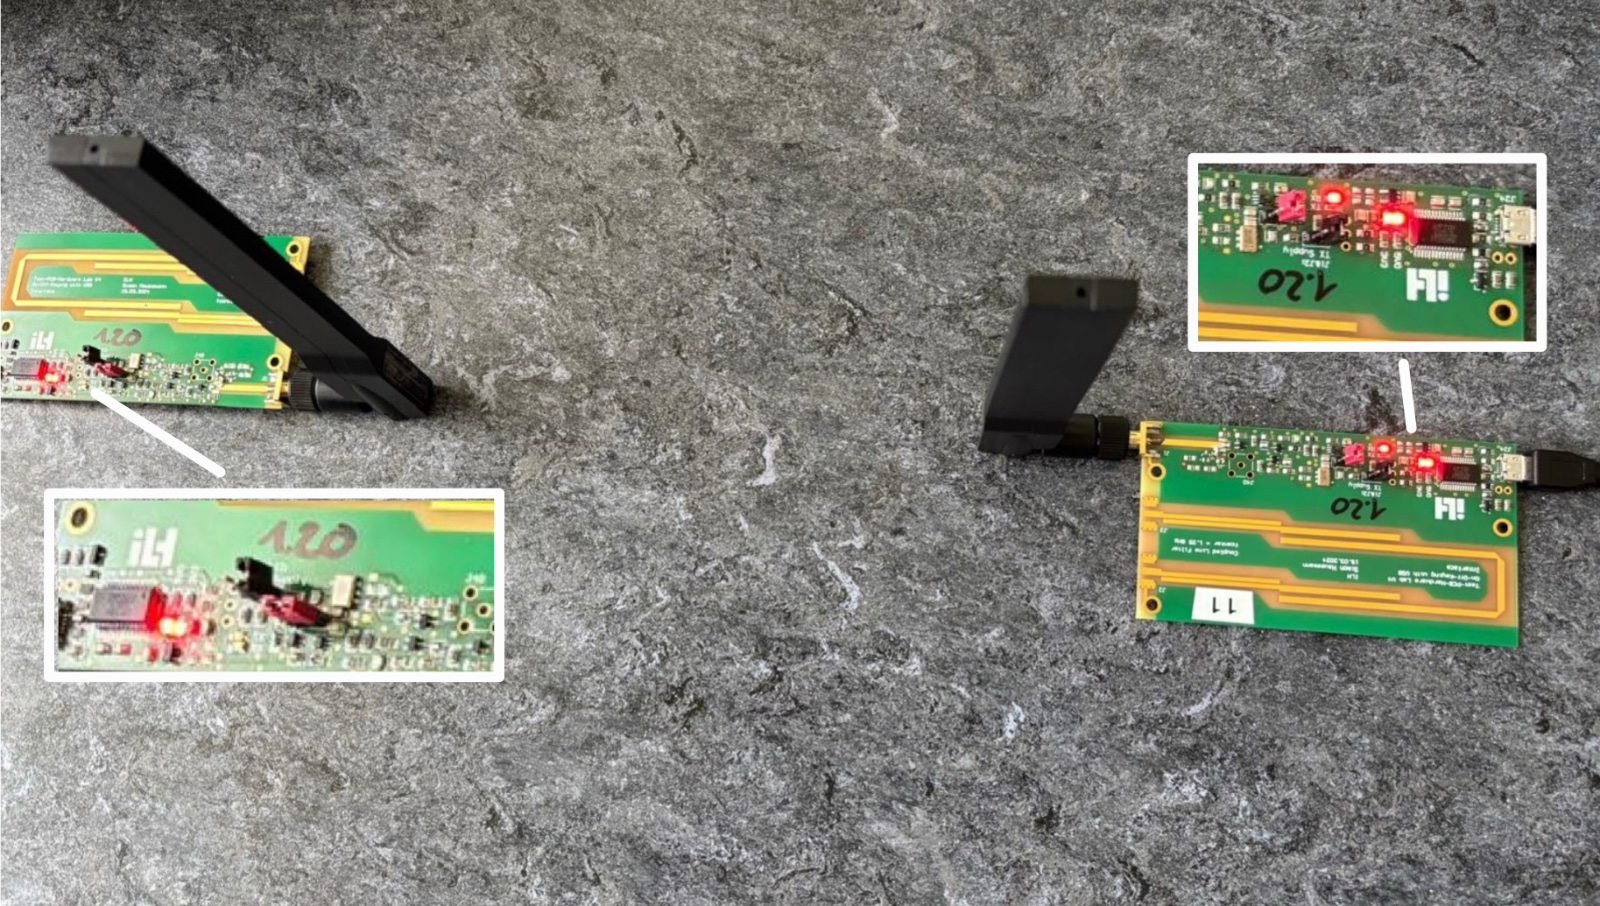
\includegraphics[width=0.8\textwidth]{Pictures/Task2a.png}
    \caption{Sender und Empfänger innerhalb der Funkreichweite}
    \label{fig:Task2a}
\end{figure}

\begin{figure}[H]
    \centering
    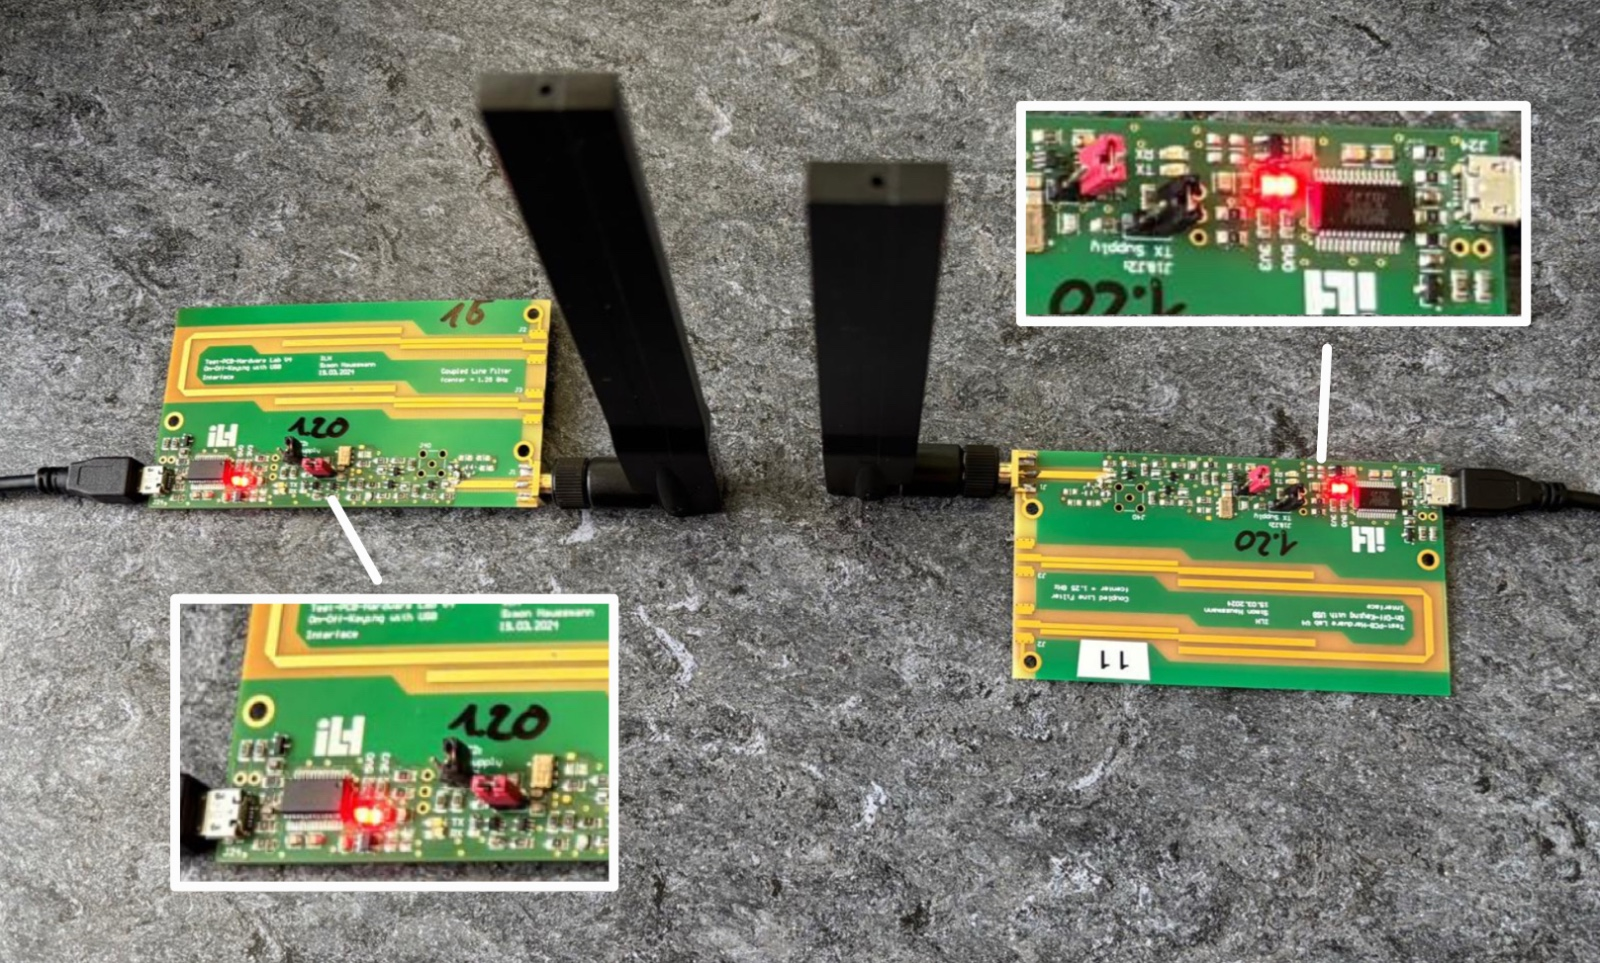
\includegraphics[width=0.8\textwidth]{Pictures/Task2aa.png}
    \caption{Sender und Empfänger außerhalb der Funkreichweite}
    \label{fig:Task2aa}
\end{figure}
Nun betrachten wir die Funkreichweite der Platinen genauer. Diese Messung führen wir auf zwei unterschiedliche
Arten durch. Einmal wird der Abstand der beiden Antennen innerhalb der Funkreichweiter erhöht bis der Kontakt
abbricht. Dann wird der Abstand der Antennen außerhalb der Funkreichweite verringert bis der Kontakt wieder
hergestellt ist. Zuerst wurd eine Funkreichweite von $d_{TR,1}=9cm$ gemessen. Auf die zweite Art wurde eine
Funkreichweite von $d_{TR,2}=8cm$ gemessen. Dies kann auf das Schwellverhalten des Empfängers (Hysterese-Effekt)
zurückzuführen sein (Evtl. erwähnung in Grundlagen). 
Ein schwaches Signal kann noch von der Platine B empfangen werden, wobei die Verbindung zu unzureichend ist um 
initial erkannt zu werden.\\
Die mindest Funkreichweite der Platinen um Signale auszuwerten beträgt somit $d_{TR,min}=8cm$.

\subsection{Plantinen am Computer anschließen}
Nur wurde die Eine Platine am Computer angeschlossen und die andere Platine an den Laptop.
Mithilfe von Hterm werden Daten in Form von ASCII von der einen Platine an die andere gesendet.
Und mit Hterm wieder ausgelesen.
Wichtig in dieser Prozedur war das verbinden beider Jumper an der Sender Platine und das entfernen beider
Jumper an der Empfänger Platine. 
Wären die Jumper bei der Empfänger Platine verbunden gewesen, wäre das problem das die Platine auch 
ein Signal gesendet hätte und dieses auch wieder empfangen hätte